% LTeX: language=fr
% Copyright © 2023, Loïc Grobol <loic.grobol@gmail.com>
% This document is available under the terms of the Creative Commons Attribution 4.0 International License (CC BY 4.0) (https://creativecommons.org/licenses/by/4.0/)

% Settings
\newcommand\myname{L. Grobol}
\newcommand\mylab{MoDyCo, Université Paris Nanterre}
\newcommand\pdftitle{Apprentissage Automatique : ???}
\newcommand\mymail{lgrobol@parisnanterre.fr}
\newcommand\titlepagetitle{\pdftitle}
\newcommand\eventname{M2 Plurital}
\newcommand\eventvenue{Nanterre, France}
\newcommand\eventdate{2024-10-16}

\documentclass[
	xcolor={svgnames},
	aspectratio=169,
	french,
]{beamer}
% Colour palettes from [Paul Tol's technical note](https://personal.sron.nl/~pault/data/colourschemes.pdf) v3.1
% Bright scheme
\definecolor{sronbrightblue}{RGB}{68, 119, 170}
\definecolor{sronbrightcyan}{RGB}{102, 204, 238}
\definecolor{sronbrightgreen}{RGB}{34, 136, 51}
\definecolor{sronbrightyellow}{RGB}{204, 187, 68}
\definecolor{sronbrightred}{RGB}{238, 102, 119}
\definecolor{sronbrightpurple}{RGB}{170, 51, 119}
\definecolor{sronbrightgrey}{RGB}{187, 187, 187}

% Divergent colour scheme (fig 19 in Paul Tol's note)
\definecolor{ptolD01}{RGB}{232,236,251}
\definecolor{ptolD02}{RGB}{217,204,227}
\definecolor{ptolD03}{RGB}{209,187,215}
\definecolor{ptolD04}{RGB}{202,172,203}
\definecolor{ptolD05}{RGB}{186,141,180}
\definecolor{ptolD06}{RGB}{174,118,163}
\definecolor{ptolD07}{RGB}{170,111,158}
\definecolor{ptolD08}{RGB}{153,79,136}
\definecolor{ptolD09}{RGB}{136,46,114}
\definecolor{ptolD10}{RGB}{25,101,176}
\definecolor{ptolD11}{RGB}{67,125,191}
\definecolor{ptolD12}{RGB}{82,137,199}
\definecolor{ptolD13}{RGB}{97,149,207}
\definecolor{ptolD14}{RGB}{123,175,222}
\definecolor{ptolD15}{RGB}{78,178,101}
\definecolor{ptolD16}{RGB}{144,201,135}
\definecolor{ptolD17}{RGB}{202,224,171}
\definecolor{ptolD18}{RGB}{247,240,86}
\definecolor{ptolD20}{RGB}{246,193,65}
\definecolor{ptolD22}{RGB}{241,147,45}
\definecolor{ptolD24}{RGB}{232,96,28}
\definecolor{ptolD25}{RGB}{230,85,24}
\definecolor{ptolD26}{RGB}{220,5,12}
\definecolor{ptolD27}{RGB}{165,23,14}
\definecolor{ptolD28}{RGB}{114,25,14}
\definecolor{ptolD29}{RGB}{66,21,10}

\definecolor{sronmutedindigo}{RGB}{51,34,136}

% And my favourite purple
\definecolor{myfavouritepurple}{RGB}{113, 10, 186}
\definecolor{electricindigo}{RGB}{111, 0, 255}
\definecolor{neonpink}{RGB}{255, 68, 204}


\usetheme[
	sectionpage=progressbar,
	subsectionpage=progressbar,
	progressbar=frametitle,
]{metropolis}
	\colorlet{accent}{neonpink}
	\setbeamercolor{frametitle}{
		use=normal text,
		bg=normal text.bg,
		fg=accent,
	}
	\setbeamercolor{alerted text}{fg=accent}
	\setbeamercolor{progress bar}{fg=accent}
	\makeatletter
		\setlength{\metropolis@progressinheadfoot@linewidth}{0.5pt}
	\makeatother

% Left-align description lists
\defbeamertemplate{description item}{align left}{\insertdescriptionitem\hfill}
\setbeamertemplate{description item}[align left]

% Use non-standard fonts
\usepackage{fontspec}
	\usefonttheme{professionalfonts}

	\directlua{
		luaotfload.add_fallback(
			"myfallback",
			{
				"NotoColorEmoji:mode=harf;",
				"NotoSans:mode=harf;",
				"DejaVuSans:mode=harf;",
			}
		)
	}
	
	\setsansfont{Fira Sans}[
		BoldFont={* Semibold},
		RawFeature={fallback=myfallback;multiscript=auto;},
	]
	\setmonofont[Scale=0.9]{Fira Mono}
	\newfontfamily\fallbackfont{Deja Vu Sans}
	\newfontfamily\emojifont{Noto Color Emoji}[Renderer=HarfBuzz]
	\frenchspacing

% Fix missing glyphs in Fira by delegating to polyglossia/babel
\usepackage{newunicodechar}
	\newunicodechar{ }{~}   % U+202F NARROW NO-BREAK SPACE
	\newunicodechar{ }{ }   % U+2009 THIN SPACE

% Notes on left screen
% \usepackage{pgfpages}
% \setbeameroption{show notes on second screen=left}

\usepackage{polyglossia}
	\setmainlanguage[variant=british]{english}
	\setotherlanguage{french}
	\setotherlanguage{breton}
	\NewDocumentCommand\borrowing{ m m }{
		\textlang{#1}{\textit}	
	}
\usepackage{amsfonts,amssymb}
\usepackage{amsmath,amsthm}
\usepackage{mathtools}	% AMS Maths service pack
	\newtagform{brackets}{[}{]}	% Pour des lignes d'équation numérotées entre crochets
	\mathtoolsset{showonlyrefs, showmanualtags, mathic}	% affiche les tags manuels (\tag et \tag*) et corrige le kerning des maths inline dans un bloc italique voir la doc de mathtools
	\usetagform{brackets}	% Utilise le style de tags défini plus haut
\usepackage{lualatex-math}

\usepackage[math-style=french]{unicode-math}
	\setmathfont[Scale=1.3]{Libertinus Math}
\usepackage{newunicodechar}
	\newunicodechar{√}{\sqrt}
\usepackage{mleftright}

% Fix incompatibility with unicode-math
\let\UnicodeMathMathBfSfIt\mathbfsfit
\let\mathbfsfit\relax
\usepackage{mismath}
\let\mathbfsfit\UnicodeMathMathBfSfIt

\usepackage{covington}
\usepackage{tabularx}
\usepackage{booktabs}
\usepackage{siunitx}
	\sisetup{
		detect-all,
		group-separator=\text{\,},
	}
	\DeclareSIUnit{\quantity}{\relax}
	\DeclareSIUnit{\words}{words}
	\DeclareSIUnit{\sentences}{sentences}
	% Needed for italics and bold numbers in siunitx S-aligned columns
	\robustify\itshape
	\robustify\bfseries
\usepackage{multicol}
\usepackage{ccicons}
\usepackage{bookmark}
\usepackage{caption}
	\captionsetup{skip=1ex, labelformat=empty}
\usepackage{lua-ul}
% \usepackage{minted}
% 	\usemintedstyle{lovelace}
% 	\setminted{autogobble, fontsize=\normalsize, tabsize=4}
% 	\setmintedinline{fontsize=auto}
% 	\RenewDocumentCommand\listingscaption{}{Example} 

\usepackage[
	english=american,
	french=guillemets,
	autostyle=true,
]{csquotes}
	\renewcommand{\mkbegdispquote}[2]{\itshape\let\emph\textbf}
	% Like `\foreignquote` but use the outside language's quotes not the inside's
	\NewDocumentCommand\quoteforeign{m m}{\enquote{\textlang{#1}{\textit{#2}}}}

\usepackage{tikz}
	\NewDocumentCommand\textnode{O{}mm}{
		\tikz[remember picture, baseline=(#2.base), inner sep=0pt]{\node[#1] (#2) {#3};}
	}
	\NewDocumentCommand\mathnode{O{}mm}{
		\tikz[remember picture, baseline=(#2.base), inner sep=0pt]{\node[#1] (#2) {\(\displaystyle #3\)};}
	}
	% Beamer utilities
	\tikzset{
		alt/.code args={<#1>#2#3}{%
		  \alt<#1>{\pgfkeysalso{#2}}{\pgfkeysalso{#3}} % \pgfkeysalso doesn't change the path
		},
		invisible/.style={opacity=0},
		visible on/.style={alt={<#1>{}{invisible}}},
		accent on/.style={alt={<#1>{draw=accent, text=accent, thick}{draw}}},
	}
	% Misc utilities
	\tikzset{
		true scale/.style={scale=#1, every node/.style={transform shape}},
	}
	% Custom styles
	\tikzset{
		>=stealth,
		hair lines/.style={line width = 0.05pt, lightgray},
		accent on/.style={alt={<#1>{draw=accent, text=accent, thick}{draw}}},
		true scale/.style={scale=#1, every node/.style={transform shape}},
	}	

	\usetikzlibrary{tikzmark}
	\usetikzlibrary{matrix, chains, graphs, graphdrawing}
	\usetikzlibrary{shapes, shapes.geometric}
	\usetikzlibrary{decorations.pathreplacing}
	\usetikzlibrary{decorations.pathmorphing}
	\usetikzlibrary{positioning, calc, intersections}
	\usetikzlibrary{fit}

% % Highlight formulas
% \usepackage[beamer, markings]{hf-tikz}

% \usepackage{forest}
% 	\useforestlibrary{linguistics}

% \usepackage{tikz-dependency}

% Plots
\usepackage{pgfplots}
	\pgfplotsset{compat=1.18}
	% Due to pgfplots meddling with pgfkeys, we have to redefine alt here.
	\pgfplotsset{
		alt/.code args={<#1>#2#3}{%
		\alt<#1>{\pgfkeysalso{#2}}{\pgfkeysalso{#3}} % \pgfkeysalso doesn't change the path
		},
	}
	\pgfplotsset{compat=1.18}
	\pgfplotsset{colormap={SRON}{rgb255=(61,82,161) rgb255=(255,250,210) rgb255=(174,28,62)}} % chktex 36

% \usepackage{robust-externalize}

	% \robExtConfigure{
	% 	add to preset={tikz}{
	% 	% we load some packages that will be loaded by figures based on the tikz preset
	% 	add to preamble={\usepackage{pifont}}
	% 	}
	% }

\usepackage[
	block=ragged,
	dashed=false,
	doi=false,
	isbn=false,
	maxbibnames=6,
	maxcitenames=2,
	minbibnames=1,
	mincitenames=1,
	uniquelist=false,
	useprefix=true,
	style=authoryear,
]{biblatex}
	% No small caps in french bib
	\DefineBibliographyExtras{french}{\restorecommand\mkbibnamefamily}
	\AtEveryBibitem{
		\ifentrytype{online}
		{} {
			\iffieldequalstr{howpublished}{online}
			{
				\clearfield{howpublished}
			} {
				\clearfield{urlyear}\clearfield{urlmonth}\clearfield{urlday}
			}
		}
	}
	% Fix bug with \insertbiblabel in author-date, see https://tex.stackexchange.com/questions/585635/beamer-biblatex-authoryear-causes-problem-with-insertbiblabel and https://github.com/josephwright/beamer/blob/865a19d4ec64f4c8e4935c19e162b8f4fd5aa190/base/beamerbaselocalstructure.sty#L501
	\let\insertbiblabel\relax
	\addbibresource{biblio.bib}
 
% Compact bibliography style
\setbeamertemplate{bibliography item}[text]

\AtEveryBibitem{
	\clearfield{series}
	\clearfield{pages}
	\clearname{editor}
}
\renewcommand*{\bibfont}{\tiny}

\usepackage{hyperxmp}	% XMP metadata

\usepackage[type={CC},modifier={by},version={4.0}]{doclicense}

% \usepackage{todonotes}
% 	\let\todox\todo
% 	\renewcommand\todo[1]{\todox[inline]{#1}}

\title{\titlepagetitle}
\author{\textbf{\myname}~(\mylab)}
\institute{}
\date{\eventname\\\eventvenue, \eventdate}

\titlegraphic{\ccby}

% Commands spécifiques
\NewDocumentCommand\shorturl{ O{https} O{://} m }{%
	\href{#1#2#3}{\nolinkurl{#3}}%
}

\DeclarePairedDelimiterX\compset[2]{\lbrace}{\rbrace}{#1\,\delimsize|\,#2}
\DeclarePairedDelimiterX\innprod[2]{\langle}{\rangle}{#1\,\delimsize|\,#2}

% Easy column vectors \vcord{a,b,c} ou \vcord[;]{a;b;c}
% Here be black magic
\ExplSyntaxOn % chktex 1
	\NewDocumentCommand{\vcord}{O{,}m}{\vector_main:nnnn{p}{\\}{#1}{#2}}
	\NewDocumentCommand{\tvcord}{O{,}m}{\vector_main:nnnn{psmall}{\\}{#1}{#2}}
	\seq_new:N\l__vector_arg_seq
	\cs_new_protected:Npn\vector_main:nnnn #1 #2 #3 #4{
		\seq_set_split:Nnn\l__vector_arg_seq{#3}{#4}
		\begin{#1matrix}
			\seq_use:Nnnn\l__vector_arg_seq{#2}{#2}{#2}
		\end{#1matrix}
	}
\ExplSyntaxOff % chktex 1

\NewDocumentCommand\itpause{}{%
	\addtocounter{beamerpauses}{-1}%
	\pause%
}

\NewDocumentCommand\graphdot{O{fill=ptolD10} r() O{0.5ex}}{\path[#1] (#2) circle (#3)}


% ██████   ██████   ██████ ██    ██ ███    ███ ███████ ███    ██ ████████
% ██   ██ ██    ██ ██      ██    ██ ████  ████ ██      ████   ██    ██
% ██   ██ ██    ██ ██      ██    ██ ██ ████ ██ █████   ██ ██  ██    ██
% ██   ██ ██    ██ ██      ██    ██ ██  ██  ██ ██      ██  ██ ██    ██
% ██████   ██████   ██████  ██████  ██      ██ ███████ ██   ████    ██

\begin{document}
\pdfbookmark[2]{Title}{title}

\begin{frame}[plain]
	\titlepage
\end{frame}

\section{Failure modes}

\begin{frame}{Specification gaming}
	From \textcite{krakovna2018SpecificationGamingExamples}

	\pause

	\begin{itemize}[<+->]
		\item \href{https://www.youtube.com/watch?v=tlOIHko8ySg}{\alert{A boat race agent}} \enquote{goes in a circle hitting the same targets instead of finishing the race.}
		\item \enquote{A robotic arm trained to slide a block to a target position on a table achieves the goal by moving the table itself.}
		\item \enquote{[Tetris] Agent pauses the game indefinitely to avoid losing.}
		\item \enquote{Deep learning model to detect pneumonia in chest x-rays works out which x-ray machine was used to take the picture; that, in turn, is predictive of whether the image contains signs of pneumonia, because certain x-ray machines (and hospital sites) are used for sicker patients.}
		\item \enquote{Agent kills itself at the end of level 1 to avoid losing in level 2}
	\end{itemize}
\end{frame}

\begin{frame}{Pourquoi tant de haine}
	Rappelez-vous du cours d'introduction :

	\pause

	L'apprentissage automatique n'a quasiment rien à voir avec l'apprentissage humain.

	\pause

	Ce n'est donc pas que les modèles ici sont malicieux ou quelque autre qualité humaine. Il existe simplement des \alert{régularités} dans les données (dans des cas assez particuliers ici), qui sont suffisamment évidentes pour être repérées et utilisées.

	\pause

	Pour un⋅e humain⋅e, la différence entre exploiter un bug et effectuer légitimement la tâche est claire. Pour un algo d'apprentissage, \alert{c'est exactement la même chose}.

	\pause

	{\small Par contre l'histoire des tanks a bien l'air apocryphe, voir \textcite{branwen2019NeuralNetTank}}
\end{frame}

\begin{frame}[standout]
	Démo : un modèle de détection d'opinions
\end{frame}

\section{Diversity ?}

\begin{frame}{Machine translation for Breton}
	\quoteforeign{breton}{Ar yezh ma ra ganti un den a zo anezhi ur bed ma vev ha ma striv ennañ}

	\quoteforeign{french}{La langue que quelqu'un pratique est un monde dans lequel il vit et lutte.}

	\only<+>{
		\begin{description}
			\item[Apertium] \quoteforeign{french}{La langue si elle fait avec elle une personne elle l'est un monde s'il vit et mon effort dans lui.} (\textcite{tyers2010RulebasedBretonFrench}, rule based)
			\item[m2m100] \quoteforeign{french}{C’est le cas d’un homme qui a laissé le coucher, et qui a laissé le coucher.} (\textcite{fan2021EnglishcentricMultilingualMachine}, multiling NMT)
		\end{description}
	}
	\only<+>{
		\begin{description}
			\item[OPUS-celtic] \enquote{The language if she has a man who lives a world and has my straight.}
			\item[OPUS-elg] \enquote{This language contains one or more people who have their own world!}
		\end{description}
	}
\end{frame}

\begin{frame}[standout]
	So what's happening?
\end{frame}


\begin{frame}{OPUS}
	OPUS \parencite{tiedemann2012ParallelDataTools} is a meta parallel corpus with covering for ≈\num{400} languages.

	For Breton, it includes most of the publicly available data:

	\begin{description}
		\item[br-fr] \qty{1.6}{\mega\sentences}
		\item[br-en] \qty{1.1}{\mega\sentences}
	\end{description}

	\pause

	\alert{BUT}
\end{frame}

\begin{frame}{Something's wrong with OPUS}
	\onslide<+->
	Most of the Breton data in OPUS comes from
	
	\begin{itemize}
		\item WikiMatrix \parencite{schwenk2021WikiMatrixMining135M}
		\item CCMatrix \parencite{schwenk2021CCMatrixMiningBillions}
		\item CCAligned \parencite{el-kishky2020CCAlignedMassiveCollection}
	\end{itemize}

	all built from parallel corpus mining:

	\onslide<+->

	\begin{enumerate}
		\item Train a \enquote{language-agnostic} vector sentence representation model e.g. LASER, \parencite{artetxe2019MassivelyMultilingualSentence}
		\item Look in monolingual corpora for sentences in different languages but with similar representations.
	\end{enumerate}

	\onslide<+->
	
	Only one corpus is actually made of human translations: OPAB (\textlang{breton}{Ofis Publik ar Brezhoneg}, \textcite{tyers2009RuleBasedAugmentationTraining}).
\end{frame}

\begin{frame}<-3>[label=opus]{Something's wrong with OPUS}
	\onslide<+->
	But: the embeddings for Breton are \alert{poorly aligned}.

	\begin{itemize}
		\item \textcite{artetxe2019MassivelyMultilingualSentence} report an \alert{error rate of \qty{85}{\percent}}!
		\item Not a surprise! It's trained using the OpenSubtitles Corpus \parencite{lison2016OpenSubtitles2016ExtractingLarge}:
			\begin{itemize}
				\item<+-> Small for Breton-* pairs.
				\item<+-> Poorly aligned.
			\end{itemize}
	\end{itemize}

	\onslide<+->
	\alert{No one has actually checked it.}
\end{frame}

\begin{frame}{What's wrong with OPUS}
	\begin{itemize}
		\item \quoteforeign{breton}{Super-harozed.} vs. \enquote{Vous êtes des héros. Des Super héros.}
		\item \quoteforeign{breton}{C'hoant 'moa goût petra 'oa c'hoarvezet.} vs. \quoteforeign{french}{J'aimais Tony. Je voulais savoir ce qui s'est passé.}
		\item \quoteforeign{breton}{Me ivez !} vs. \enquote{What are the chances?}
		\item \quoteforeign{breton}{Kae da sutal, Pakistan brein !} vs. \enquote{You're sorry?}
	\end{itemize}
\end{frame}

\againframe<3->{opus}

\begin{frame}[standout]
	No speaker of Breton has ever been involved in the development of either datasets or models.	
\end{frame}

\subsection{Other crimes}

\begin{frame}{GPT 3.5}
	\quoteforeign{breton}{Ar yezh ma ra ganti un den a zo anezhi ur bed ma vev ha ma striv ennañ}

	\quoteforeign{french}{La langue que quelqu'un pratique est un monde dans lequel il vit et lutte.}

	\begin{description}
		\item[GPT-3.5] \quoteforeign{french}{La langue qu'elle parle est celle d'une personne qui a en elle un monde où elle vit et lutte.}
	\end{description}
\end{frame}

\begin{frame}{GPT 3.5}
	\quoteforeign{french}{La langue que quelqu'un pratique est un monde dans lequel il vit et lutte.}
	
	\quoteforeign{breton}{Ar yezh ma ra ganti un den a zo anezhi ur bed ma vev ha ma striv ennañ.}

	\begin{description}
		\item<+->[GPT-3.5] \quoteforeign{breton}{An teunga a implij ur vro eo ur bed en e ober a blij ha emdroadur.}
		\item<+->[GPT-3.5] \quoteforeign{breton}{Yezh mae eun an hini a labour, ur bed e vev ha ober a raio.}
		\item<+->[GPT-3.5] \quoteforeign{breton}{Yezh ar re a labour a zo bed ma vev ha ma c'hevrioù.}
		\item<+->[GPT-3.5] …
	\end{description}	
\end{frame}

\begin{frame}[plain]
	\begin{overprint}
		\onslide<+>
			\centerline{
				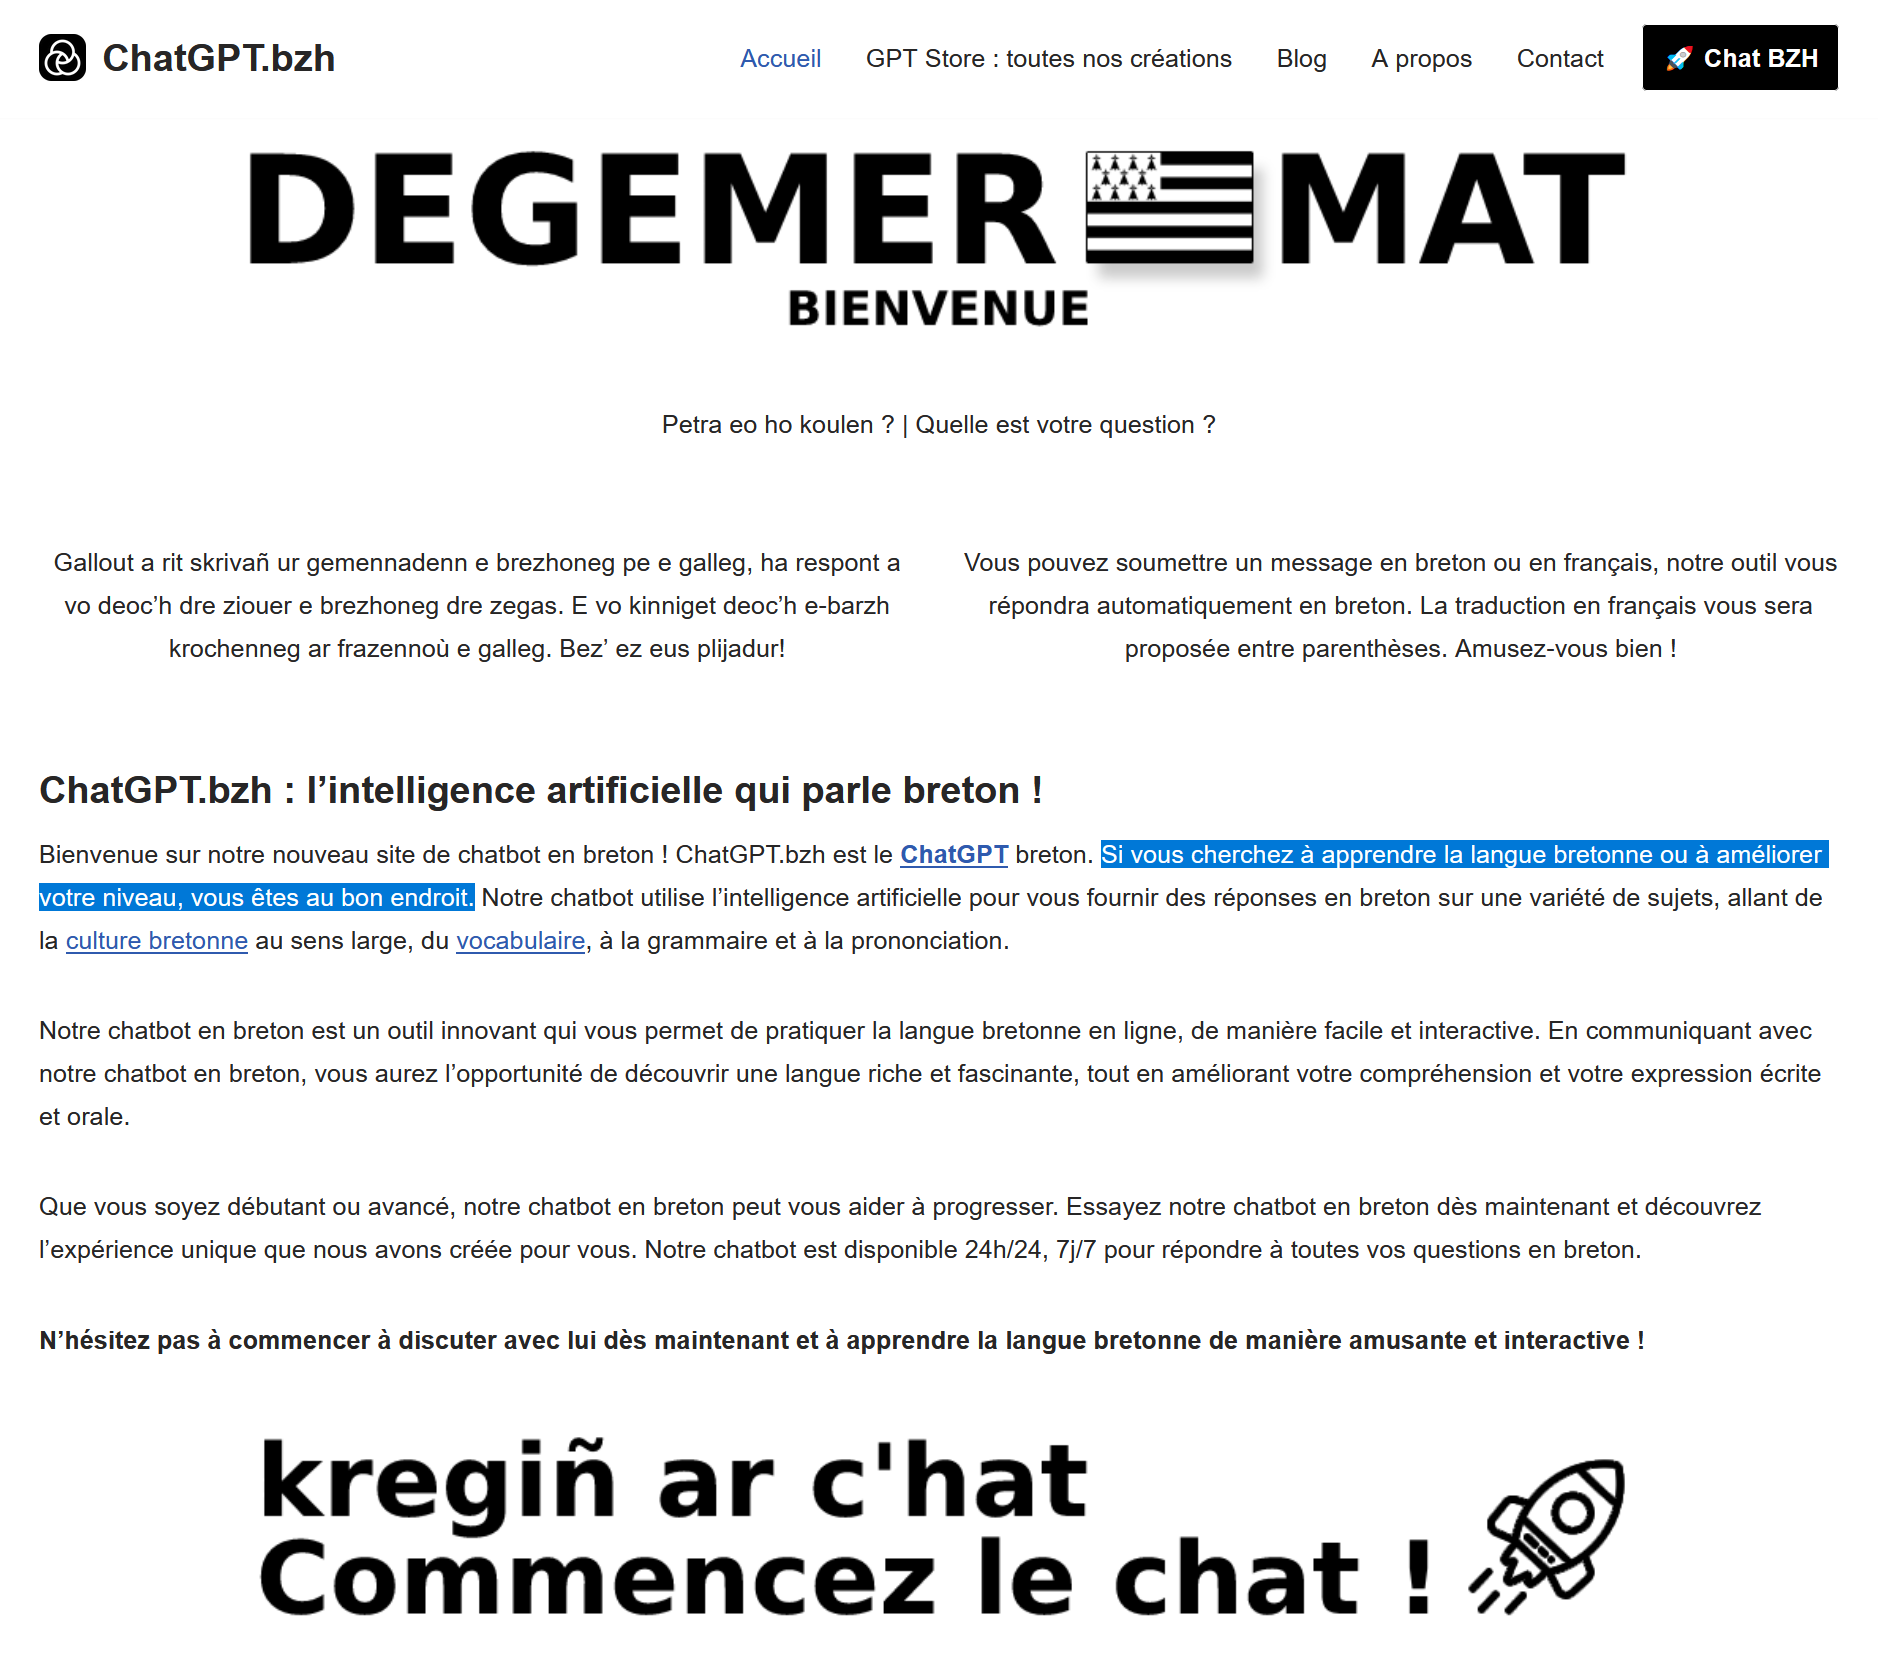
\includegraphics[width=1\textwidth,height=\textheight, keepaspectratio]{pics/couturier 24.03.2024 - frontpage.PNG}
			}
		\onslide<+>
			\centerline{
				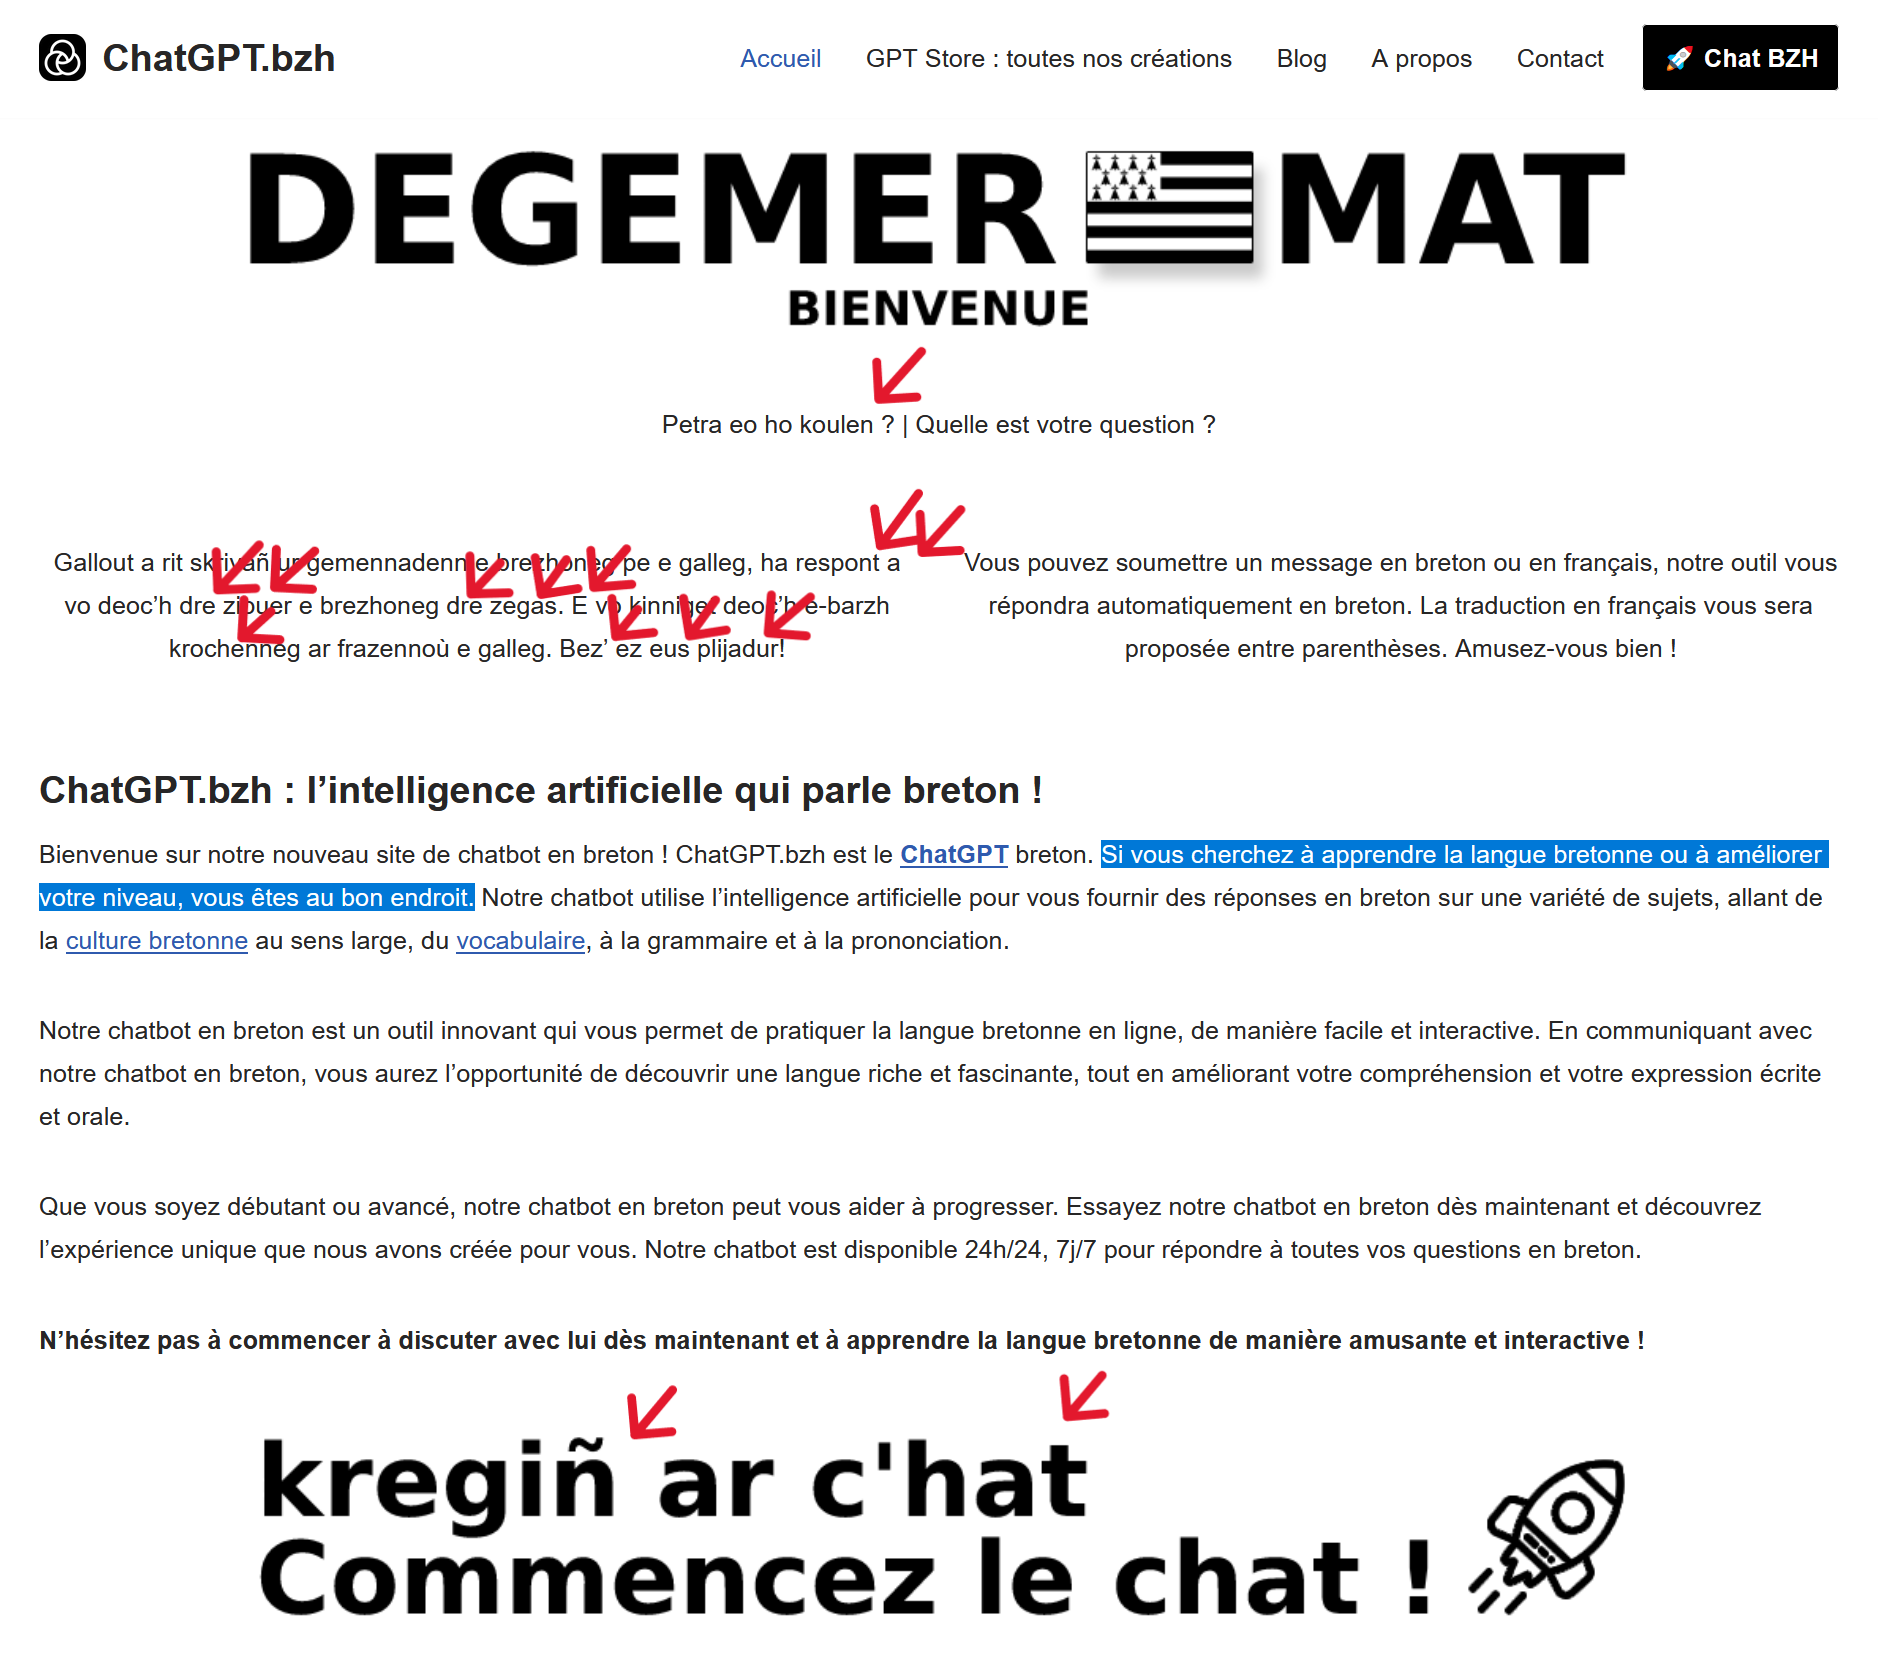
\includegraphics[width=1\textwidth,height=\textheight, keepaspectratio]{pics/couturier 24.03.2024 - frontpage - fautes marquees.PNG}
			}				
	\end{overprint}
\end{frame}

\subsection{With a little help from field linguistics}

\begin{frame}[plain]
	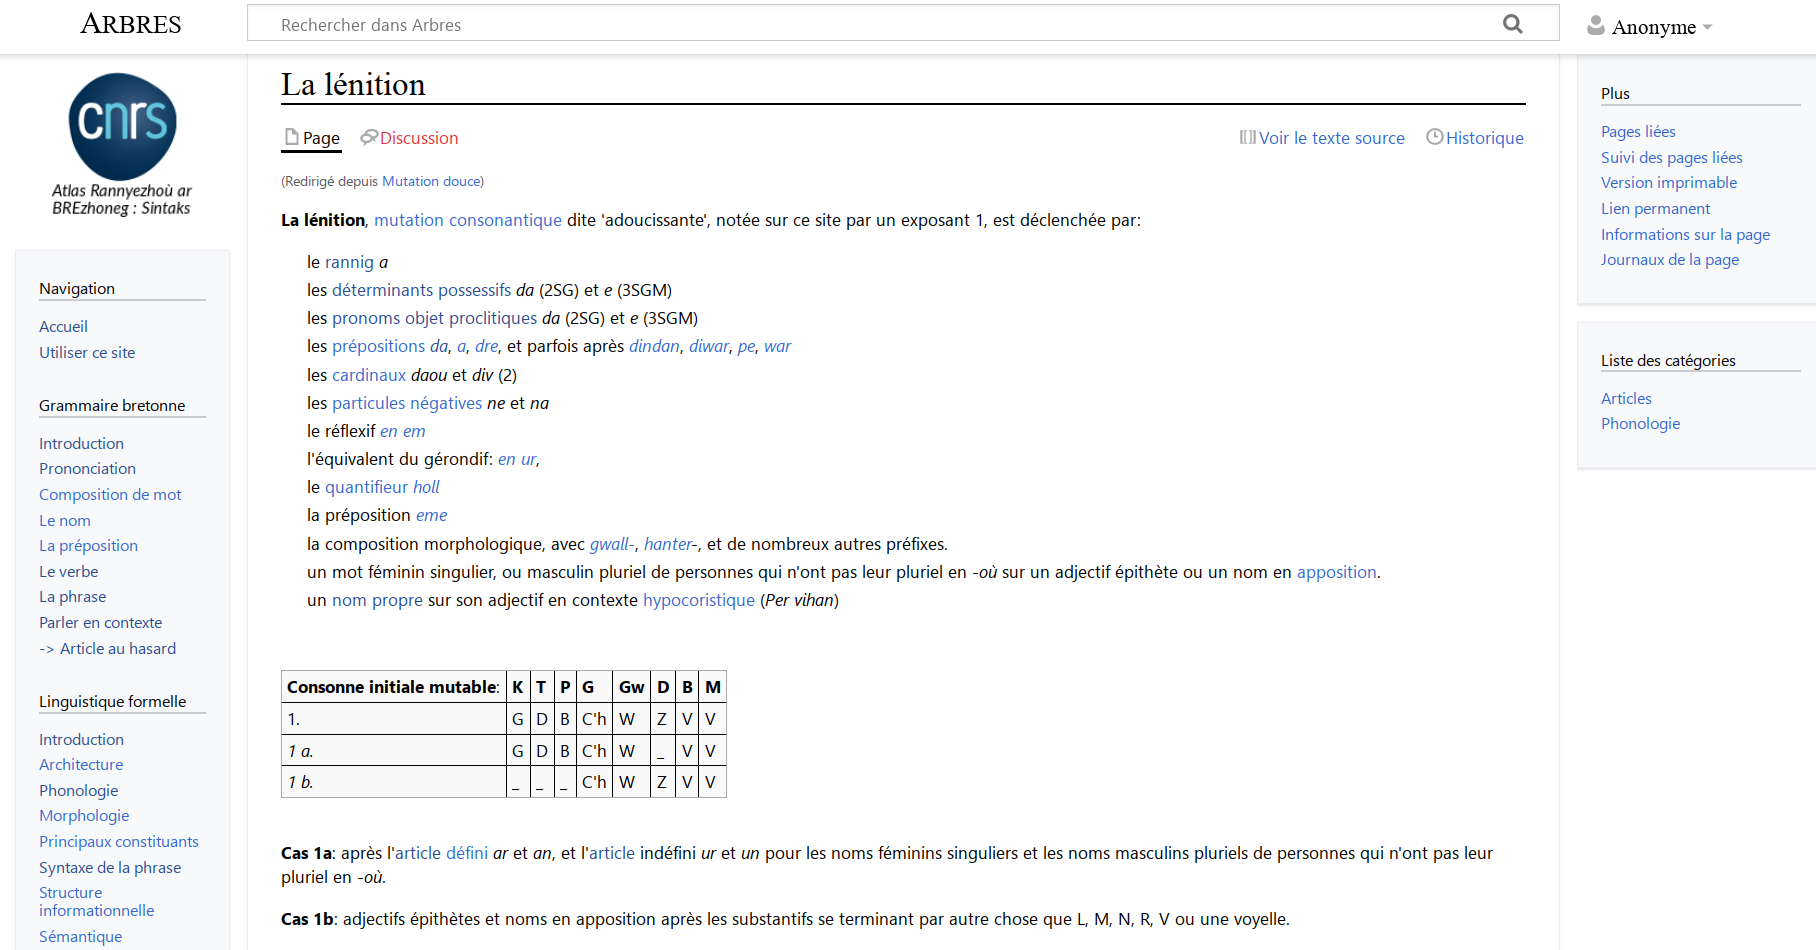
\includegraphics[width=1.1\textwidth]{pics/arbres.png}
\end{frame}

\begin{frame}{Wikigrammar}
	\textlang{breton}{\textbf{A}tlas \textbf{R}annyezhoù ar \textbf{BRE}zhoneg: \textbf{S}intaks} \parencite{jouitteau2009ARBRESWikigrammaireDialectes}
	\begin{itemize}
		\item A public, collaborative and evolutive \alert{research notebook} for fundamental research in formal linguistics.
		\item A descriptive \alert{grammar for the speaking community}.
		\item Including \alert{illustrative data}
			\begin{itemize}
				\item News
				\item Cultural/artistic productions
				\item Social media content
				\item \alert{Elicitation} data collected in linguistic \alert{fieldwork}
			\end{itemize}
	\end{itemize}
\end{frame}

\begin{frame}{ARBRES Kenstur}
	\onslide<+->
	Breton sentences and their translations extracted from ARBRES's interlinear glosses:

	\begin{covexample}
		\digloss{
			eur 	mell 	gwezenn 	glas 	he 	deliou
		}{
			a 	big 	tree.SG 	green 	his\textsuperscript{2} 	leaf.PL
		}{
			a big tree with green leaves
		}
	\end{covexample}
\end{frame}

\begin{frame}{Volume}
	\onslide<+->
	After extraction and deduplication we got \alert{\qty{5192}{\sentences}}
	\begin{itemize}
		\item<+->[→] An order of magnitude less than the \emph{\textlang{breton}{Ofis Publik ar Brezhoneg}} parallel corpus.
	\end{itemize}

	\onslide<+->

	So is it all for nothing?

	\onslide<+->\vfill

	No!
\end{frame}

\begin{frame}{Systems comparison}
	For a more precise comparison, we evaluate:
	
	\begin{description}
		\item[Apertium] Mostly rule-based, developed for Breton by \textcite{tyers2010RulebasedBretonFrench} on the OPAB corpus.
		\item[m2m100-418m] out-of-the-box.
		\item[+OPUS] with continued pretraining on OPUS data (with heuristic filtering for quality, so mostly OPAB)
		\item[+ARBRES] with both OPUS and ARBRES Kenstur.
	\end{description}

	Evaluation on a (sadly) for now private dataset from OPAB.
\end{frame}

\begin{frame}{Results}
	\onslide<+->
	\begin{table}[thb]
		\centering
		\begin{tabular}{l*{2}{S[table-format=2.2]}S[table-format=3.2]}
			\toprule
			{\textbf{Model}} & {\textbf{BLEU}} & {\textbf{ChrF++}} & {\textbf{TER}}\\
			\midrule
			Apertium            & 24.15 & 50.23 &  63.93\\
			m2m100-418M         & 00.58 & 11.85 & 114.49\\
			\quad +OPAB         & 30.01 & 50.16 &  55.37\\
			\quad\quad +ARBRES  & 37.68 & 56.99 &  48.65\\
			\quad +Korpus Nevez & 40.37	& 59.14	&  44.10\\
			\bottomrule
		\end{tabular}
		\caption{Evaluation results on the OPAB test dataset.}
	\end{table}
	\onslide<+->

	\begin{itemize}
		\item Apertium fares surprisingly well
		\item Despite the limited size of ARBRES, the gain is important.
		\item<+-> ALSO LOOK AT THAT LAST LINE OMG
	\end{itemize}
\end{frame}

\begin{frame}{But what does it look like?}
	\quoteforeign{breton}{Ar yezh ma ra ganti un den a zo anezhi ur bed ma vev ha ma striv ennañ}

	\quoteforeign{french}{La langue que quelqu'un pratique est un monde dans lequel il vit et lutte.}

	\begin{description}
		\item[m2m100] \quoteforeign{french}{C’est le cas d’un homme qui a laissé le coucher, et qui a laissé le coucher.}
		\item[+OPUS] \quoteforeign{french}{La langue dans laquelle elle fait un homme est un monde dans lequel elle vit et s'efforce.}
		\item[+OPUS+ARBRES] \quoteforeign{french}{La langue dans laquelle un homme parle est un monde dans lequel il vit et s'efforce.}
	\end{description}	
\end{frame}

\subsection{What now?}

\begin{frame}{Why?????}
	\onslide<+->
	For companies and research institutions, there is a real incentive to \only<+->{\alert<.>{claim to}}\ handle minority languages.

	\onslide<+->
	But very little to actually do it well: doing poorly has very little consequences.
	
	\onslide<+->
	This leads to a form of \alert{diversity washing}, with plausible-ish deniability.
	
	\onslide<+->
	Whenever there is at least some data available, just use it. No need for any other commitment: \alert{the subaltern cannot speak} \parencite{chakravortyspivak1988CanSubalternSpeak}.
\end{frame}

\begin{frame}{Consequences}
	By increasing severity:
	\begin{itemize}[<+->]
		\item Proliferation of erroneous language, potentially contaminating uses of even native speakers.
		\item Hiding the lack of actual language technologies, leading to lack of investments by public actors.
		\item Linguistic conflict between NLP tools and actual speakers, furthering their dispossession and silencing.
	\end{itemize}
	
	\onslide<+->
	Worst of all: producers of such NLP tools have a direct economic inventive in silencing the linguistic communities!
	
	\onslide<+->
	In many cases, these minority linguistic communities are already in difficult positions re: literacy in English, higher education, competences in CS and linguistics, and access to media.
\end{frame}

\begin{frame}{Lessons}
	On a basic level:
	\begin{itemize}[<+->]
		\item Take claims of massive multilingualism with a big grain of salt.
		\item Be very careful with uncontrolled parallel data mining.
		\item \alert{Curating} a \alert{focused} dataset is worth the effort.
	\end{itemize}
\end{frame}

\begin{frame}{Lessons}
	More importantly:
	\begin{itemize}[<+->]
		\item NLP without \alert{language experts} makes very little sense.
		\item NLP \alert{by} language experts is a lot better. In all respects.
		\item \alert{Linguists} and their data are far too precious to ignore.
	\end{itemize}
\end{frame}

\begin{frame}{What to do}
	Most importantly:
	\begin{itemize}[<+->]
		\item Stop thinking of NLP experts, language experts and linguistic communities as separate entities.
		\item Stop thinking of NLP as a collect data → train → evaluate pipeline with separate actors.
		\item \alert{Listening} to linguistic communities is good, but it's not enough:
			\begin{itemize}[<+->]
				\item Teach.
				\item Support.
				\item \alert{Don't be an outsider}.
			\end{itemize}
	\end{itemize}
\end{frame}

\section{Mental illusions}

\begin{frame}[plain]
	\begin{center}
		\Large\alert{\url{https://www.youtube.com/watch?v=wp8ebj_yRI4}}
	\end{center}
\end{frame}

%  █████  ██████  ██████  ███████ ███    ██ ██████  ██ ██   ██
% ██   ██ ██   ██ ██   ██ ██      ████   ██ ██   ██ ██  ██ ██
% ███████ ██████  ██████  █████   ██ ██  ██ ██   ██ ██   ███
% ██   ██ ██      ██      ██      ██  ██ ██ ██   ██ ██  ██ ██
% ██   ██ ██      ██      ███████ ██   ████ ██████  ██ ██   ██

\hypersetup{bookmarksdepth=0}  % Don't create the bookmark for the Appendix part
\appendix
\hypersetup{bookmarksdepth=2}
\bookmarksetup{startatroot}
\section{Appendix}

\pdfbookmark[3]{References}{references}
\begin{frame}[allowframebreaks]{References}
	\printbibliography[heading=none]
\end{frame}

\pdfbookmark[3]{Licence}{licence}
\begin{frame}{Licence}
	\begin{english}
		\begin{center}
			{\huge \ccby}
			\vfill
			This document is distributed under the terms of the Creative Commons Attribution 4.0 International Licence (CC BY 4.0) (\shorturl{creativecommons.org/licenses/by/4.0})

			\vfill
			© 2024, L. Grobol <\shorturl[mailto][:]{loic.grobol@gmail.com}>

			\shorturl[https]{lgrobol.eu}
		\end{center}
	\end{english}
\end{frame}

\end{document}
